
\section{Visualization with GNUPlot}

\paragraph{Anzeige mit GNUPlot}
Zur Anzeige der Statistiken eines abgeschlossenen Simulationsdurchlaufes muss die entsprechende GNUPlot-Konfigurationsdatei mit GNUPlot geöffnet werden: Unter Unix-System kann man hierfür nach Aufruf von \texttt{\$ gnuplot} die interaktive GNUPlot-Shell verwenden (\texttt{> load ``gnuplotfile.plt``}). Weitere Befehle mit \texttt{> help}. Alternativ kann man sich die Ausgabe direkt anzeigen lassen mittels Shellkommando \texttt{\$ gnuplot -persist ''gnuplotfile.plt``}, wobei das \texttt{-persist} bewirkt, dass das Anzeigefenster auch nach Erstellen der Ausgabe geöffnet bleibt. Weitere Flags siehe \texttt{\$ man gnuplot}.


\paragraph{Konfiguration der Anzeige}
Der Inhalt der Datei \texttt{output\_20091224\_184129\_ALL.plt} könnte auszugsweise so aussehen:

\begin{center}
\texttt{\begin{tabular}{rrrl}
\# time & avg\_spd & minball\_x & (...) \\
\hline
0 & 9.2 & 20.5 \\
1 & 11.3 & 21.5 \\
4 & 9.1 & 21.9 \\
6 & 7.5 & 22.3
\end{tabular}}
\end{center}

Jede Zeile enthält die statistischen Daten zu einem bestimmten Zeitpunkt. Der Beginn einer neuen Spalte wird hierbei durch (mindestens) ein Leerzeichen gekennzeichnet. '\#' leitet eine Kommentarzeile ein.

In der Datei \texttt{gnuplot\_20091224\_184129\_ALL.plt} findet nun die Formatierung der Daten für die Anzeige statt und kann beliebig geändert werden:

\begin{verbatim}
# statistics of the simulation
#====================================
set title ' SCHLAUE SCHWÄRME '
set xrange []
set yrange []
set grid
set pointsize 0.5
set xlabel 'time'
set ylabel ''
plot 'output_(...)_ALL.plt' using 1:2 title 'avg_spd' with linespoints, \
     'output_(...)_ALL.plt' using 1:3 title 'minball_x' with linespoints
\end{verbatim}

Die Angaben haben folgende Bedeutung:
\begin{itemize}
\item \texttt{set title '\textit{Titel}'} erzeugt einen zentrierten Titel am oberen Teil der grafischen Darstellung.
\item \texttt{set xrange [\textit{min}:\textit{max}]} begrenzt den horizontal sichtbaren Bereich zwischen den Werten \texttt{\textit{min}} und \texttt{\textit{max}}, \texttt{set xrange []} führt diese Skalierung auf Grundlage der vorliegenden Daten automatisch durch.
\item \texttt{set grid} blendet ein Gitternetz ein.
\item \texttt{set pointsize \textit{multiplikator}} skaliert die Größe der Punkte (falls eine Darstellung gewählt wird, welche Punkte beinhaltet) gemäß \texttt{\textit{multiplikator}}.
\item \texttt{xlabel '\textit{Label}'} beschriftet die X-Achse.
\end{itemize}
Diese Angaben beinhalten also \textit{nur} grafische grafische Aspekte, die z.B. für die Verwendung in Dokumentationen angepasst werden können. Die Einstellungen der anzuzeigenden Daten finden erst daraufhin statt:

\begin{itemize}
 \item \texttt{plot '\textit{Dateiname.plt}'} leitet den tatsächlichen Vorgang der Darstellung ein. Hierbei werden die Daten aus der angegebenen Datei gelesen. Durch \texttt{using 1:2} werden die erste und die zweite Spalte gegeneinander dargestellt, wobei der erstgenannte Spaltenindex, also \texttt{time}, die X-Koordinate und folglich \texttt{avg\_spd} die Y-Koordinate definiert. \texttt{title `avg\_speed'} fügt für die definierte Funktion einen Legendeneintrag mit dem Titel \texttt{avg\_speed} hinzu. Der Zusatz \texttt{with linespoints} beschreibt die Darstellung durch mit Linien verbundene Zeichen an den Datenpunkten. \texttt{linespoints} kann auch ersetzt werden durch:
\begin{itemize}
\item \texttt{lines} verbindet jeden Datenpunkt mit einer Linie
\item \texttt{dots} zeigt einzelne Punkte an (sinnvoll bei vielen Datenpunkten)
\item \texttt{points} fügt ein Zeichen an der Position des Datenpunktes ein. Die Größe kann durch den Befehl \texttt{set pointsize} geändert werden
\item \texttt{linespoints} erstellt gleichzeitig \textit{points} und \textit{lines}
\item \texttt{impulses} erzeugt eine vertikale Linie ausgehend von der X-Achse zum Datenpunkt
\end{itemize}
Zum Plotten einer weiteren Funktion in derselben Darstellung wird die gleiche Struktur durch ein Komma getrennt angehangen (auch aus verschiedenen Quelldateien). Dies ermöglicht auf einfache Art, dass die Darstellung der Statistiken unterschiedlicher Simulationsdurchläufe in einer Grafik dargestellt werden können.
\end{itemize}

\paragraph{Ergebnis}~\\

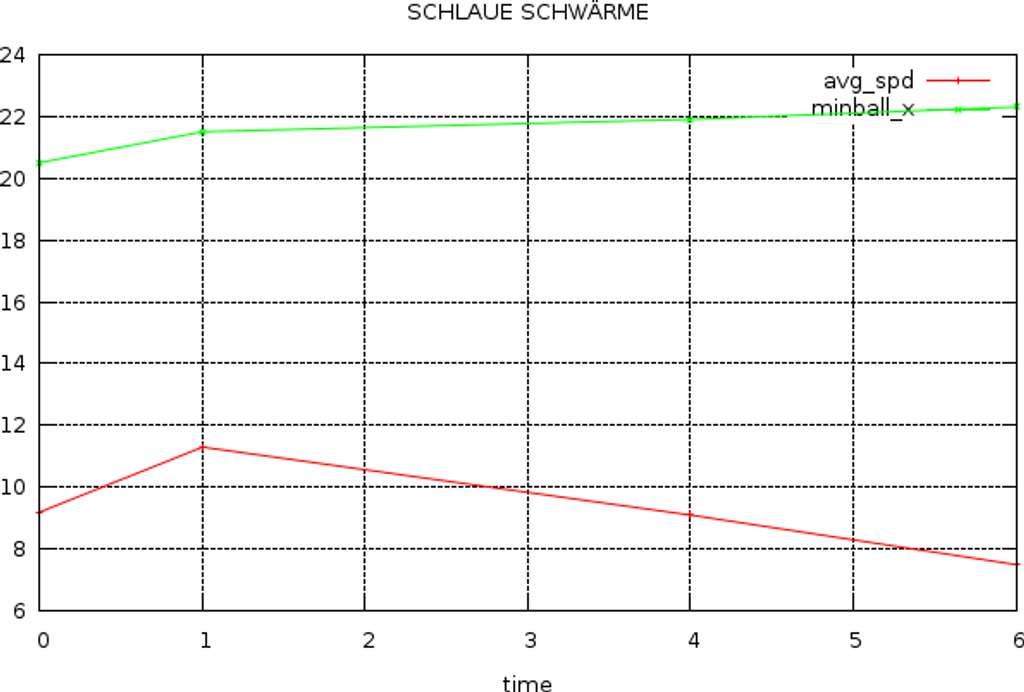
\includegraphics[width=\textwidth]{stats-howto-gnuplot.png}

\paragraph{Weitere Informationen zu GNUPlot}~\\

\begin{tabular}{l}
 $[1]$ offizielle Homepage: \url{http://www.gnuplot.info/} \\
 $[2]$ Grundkurs: \url{http://userpage.fu-berlin.de/~voelker/gnuplotkurs/gnuplotkurs.html}
\end{tabular}